\documentclass[a4paper, 11pt]{article}
\usepackage[utf8]{inputenc}
\usepackage{amsmath}
\usepackage{array}
\usepackage{amssymb} 
\usepackage{array,multirow,makecell}
\usepackage{comment}
\usepackage{fullpage} 
\usepackage{graphicx}
\usepackage{bussproofs}
\usepackage{mathtools}
\usepackage[makeroom]{cancel}
\graphicspath{ {./images/} }
\usepackage{graphicx}
\usepackage{subfig}
\usepackage{tikz} 
\usetikzlibrary{positioning}

\usepackage{tcolorbox}
\usepackage{listings}
\usepackage{xcolor}
 
\definecolor{codegreen}{rgb}{0,0.6,0}
\definecolor{codegray}{rgb}{0.5,0.5,0.5}
\definecolor{codepurple}{rgb}{0.58,0,0.82}
\definecolor{backcolour}{rgb}{0.95,0.95,0.92}
 
\lstdefinestyle{mystyle}{
    backgroundcolor=\color{backcolour},   
    commentstyle=\color{codegreen},
    keywordstyle=\color{magenta},
    numberstyle=\tiny\color{codegray},
    stringstyle=\color{codepurple},
    basicstyle=\ttfamily\footnotesize,
    breakatwhitespace=false,         
    breaklines=true,                 
    captionpos=b,                    
    keepspaces=true,                 
    numbers=left,                    
    numbersep=5pt,                  
    showspaces=false,                
    showstringspaces=false,
    showtabs=false,                  
    tabsize=2
}
 
\lstset{style=mystyle}

\newtcolorbox{mybox}[3][]
{
  colframe = #2!25,
  colback  = #2!10,
  coltitle = #2!20!black,  
  title    = {#3},
  #1,
}

\title{AML - Notes}

\begin{document}
\maketitle

\section{The basics of Semilattices}

\

\begin{tcolorbox}
    \textbf{Definition:} A binary operation $R$ in $E$ is an \textbf{order} if:
    
    \begin{itemize}
        \item $R$ is reflexive: $xRx$
        \item $R$ is anti-symetric: for any $x \in E$, and $y \in E$, if $xRy$ and $y \neq x$, then $y\cancel{R}x$.
        \item $R$ is transitive: if $xRy$ and $yRz$ then $xRz$.
    \end{itemize}
    
    \textbf{Definition:} A binary operation $R$ in $E$ is a \textbf{total order} if it is an order and:
    
    \
    
    $\forall (x,y) \in E^2 / x \neq y$: $xRy$ or $yRx$.
    
    \
    
    \textbf{Definition:} A binary operation $R$ in $E$ is a \textbf{partial order} if it is an order but not a total one.
    
    \
    
    \textbf{Definition:} If an order $R$ is not reflexive, it is a \textbf{strict order} of $E$.
    
\end{tcolorbox}

\

\begin{tcolorbox}
    \textbf{Definition:} A \underline{semilattice} is a structure $\boldsymbol{S} = <S,\cdot>$ where $\cdot$ is a binary operation, called the \underline{semilattice operation}, such that:
    
    \begin{itemize}
        \item $\cdot$ is associative: $(xy)z = x(yz)$
        \item $\cdot$ is commutative: $xy = yx$
        \item $\cdot$ is idempotent: $xx=x$
    \end{itemize}
    
\end{tcolorbox}

\

\begin{tcolorbox}
    \textbf{Definition:} Let $\boldsymbol{S}$ and $\boldsymbol{T}$ be semilattices. A \textbf{morphism} from $\boldsymbol{S}$ to $\boldsymbol{T}$ is a function $h: S \rightarrow T$ that is a homomorphism; ie:
    
    \
    
    $h(xy) = h(x)h(y)$
    
\end{tcolorbox}

\

\begin{tcolorbox}
    \textbf{Definition:} A \textbf{join-semilattice} is a structure $\boldsymbol{S} = <S,\lor>$, where $\lor$ is a binary operation, called the \textbf{join}, such that:
    
    \begin{itemize}
        \item $\leq$ is a partial order, where $x \leq y \Leftrightarrow x \lor y = y$
    \end{itemize}

\end{tcolorbox}

\

\begin{tcolorbox}
    \textbf{Definition:} A \textbf{meet-semilattice} is a structure $\boldsymbol{S} = <S,\land>$, where $\land$ is a binary operation, called the \textbf{meet}, such that:
    
    \begin{itemize}
        \item $\leq$ is a partial order, where $x \leq y \Leftrightarrow x \land y = x $
    \end{itemize}

\end{tcolorbox}

\section{The basics of AML}

\subsection{Elements of the Algebra}

\

The first paper describing AML uses semilattices to embed problems into an algebra. The binary operation is called "\textbf{merge}" (symbol $\odot$) and the set $S$ has three types of of elements: \textbf{constants, terms and atoms}.

\

Terms should describe the objects of the problem. For exemple, terms can represent images as matrices. Here's a simple exemple of a 4-pixel image described by a term $T$:

\begin{equation*}
    T = \begin{bmatrix}
    c_1 & c_2 \\
    c_3 & c_4
    \end{bmatrix}
\end{equation*}

Here $c_1, c_2, c_3$ and $c_4$ are constants, the primitive description elements of any embedding problem, and so the previous representation of $T$ in the algebra $S$ is:

\begin{equation*}
    T = c_1 \odot c_2 \odot c_3 \odot c_4
\end{equation*}

Atoms are elements created by the learning algorithm, represented by greek letters, and each constant is a merge of atoms. Here, $T$ is therefore a merge of atoms too.

\

Given that $T$ and $c_1$ are both elements of the algebra, it is clear that this algebra defines a partial order because the merge of $T$ and $c_1$ is still $T$ (ie. $T = T \odot c_1$).  We can therefore establish the inclusion relationship $<$ between elements $a$ and $b$ of the algebra:

\begin{equation}
    a < b \Leftrightarrow b = b \odot a
\end{equation}

\subsection{Training set}

The toy exemple of the article is to classify 2x2 images in which pixels can be either black or white into images having a black vertical bar and images that don't. The training data is the following:

\begin{center}
    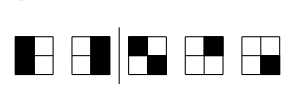
\includegraphics{training_data.png}
\end{center}

Where the two examples on the left are labeled "positive" because they have a black vertical bar (they are nammed $T_1^+$ and $T_2^+$) and the rest is labeled "negative" ($T_3^-$, $T_4^-$ and $T_5^-$) because they don't.

\

So the “training set” of the algebra consists of a set $R$ of positive and negative relations of the form
($v < T_1^+$) or $\neg(v < T_3^-)$, where $v$ is a constant, one we want to describe to our algebra
by using examples and counterexamples.

\begin{center}
    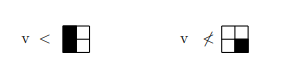
\includegraphics{training_data_w_constant.png}
\end{center}

\subsection{Graph of the algebra}

\

The graph of the algebra is a representation of the inclusion relationships we just described. The graph has nodes only for the subset of terms in the trainning data, plus 
the "pinning terms" that are calculated by the algorithm (those will be introduced later). 

\

This means that $a \rightarrow b \Rightarrow a < b$, but there is no if and only if, because not all terms should be in the graph.

\

If a term $T$ is \textit{defined} as the merge of constants $c_i$ then:

\begin{equation*}
    T = \bigodot_i c_i \Rightarrow \forall i, c_i \rightarrow T
\end{equation*}

\

If all components of a term $T$ are also components constants of another term $S$, then there is an edge between the two:

\begin{equation*}
    T < S \Rightarrow T \rightarrow S
\end{equation*}

For atoms only, we have:

\begin{equation*}
    \phi \rightarrow b \Leftrightarrow \phi < b
\end{equation*}

\

\begin{tcolorbox}
For the graph of the algebra, the \textbf{partial order $<$} is defined as:

\begin{equation}
    a < b \Leftrightarrow \forall \phi, ((\phi \not\rightarrow a) \lor (\phi \rightarrow b))
\end{equation}

where the universal quantifier runs over all atoms. 
\end{tcolorbox}

This formula states that $a < b$ if and only if all the atoms edged to $a$ are also edged to $b$; given that for each atom, either the atom is not edged to $a$ but edged to $b$ or it is not edged to both $b$ and $a$. 

\

\underline{\textbf{Proof of the partial order}}

\

i. \underline{Reflexion}.

\

Let $x$ be a node of the graph but not an atom.

$\forall \phi, (\phi \not\rightarrow x) \lor (\phi \rightarrow x) \equiv \neg(\phi \rightarrow x) \lor (\phi \rightarrow x) = \top$

\

ii. \underline{Antisymetry}:

\

Let's proove that if $a < b$ and $a \neq b$ then $b \not< a$. Or, by the definition of the relation:

\begin{center}
    for $a \neq b$, $a < b \Rightarrow (\exists \phi, \phi \not\rightarrow a \land \phi \rightarrow b)$
\end{center}

This formula means that if $a$ is included in $b$, and if $a$ is not $b$, then there must be at least one atom that $b$ has but $a$ doesn't. 

\

To proove it, we define $a$ and $b$ such that $a < b$ and $a \neq b$. Then, we suppose the negation of the right side of the implication to be true. Therefore we have, for all $\phi$:

\begin{center}
    $\phi \not\rightarrow a \lor \phi \rightarrow b$
\end{center}

and,

\begin{center}
    $\phi \rightarrow a \lor \phi \not\rightarrow b$
\end{center}

\begin{itemize}
    \item $\phi \not\rightarrow a \land \phi \rightarrow a$ and $\phi \not\rightarrow b \land \phi \rightarrow b$ is trivialy contradictory.
    \item $\phi \not\rightarrow a \land \phi \not\rightarrow b$ is impossible because each constant must be a merge of atoms.
    \item $\phi \rightarrow a \land \phi \rightarrow b$ is impossible because it would mean that $a=b$.
\end{itemize}

\

iii. \underline{Transitivity}:

\

To prove the transitivity proprety we must proove that:

\begin{equation*}
    \forall \phi, (\phi \not\rightarrow a \lor \phi \rightarrow b) \land (\phi \not\rightarrow b \lor \phi \rightarrow c) \Rightarrow (\phi \not\rightarrow a \lor \phi \rightarrow c) 
\end{equation*}

Or, it's contraposition:

\begin{equation*}
    \exists \phi, (\phi \rightarrow a \land \phi \not\rightarrow c) \Rightarrow (\phi \rightarrow a \land \phi \not\rightarrow b) \lor (\phi \rightarrow b \land \phi \not\rightarrow c) 
\end{equation*}

Let's suppose an atom $\phi$ for witch $\phi \rightarrow a \land \phi \not\rightarrow c$ exists. This means that an atom that is edged to $a$ but not edged to $c$ exists. Let's consider two cases: one where $\phi$ is edged to $b$ and one where it's not. If $\phi$ is edged to $b$, then we have $\phi \rightarrow b \land \phi \not\rightarrow c$. Therefore the contraposition is verified because of it's right term. If $\phi$ is not edged to $b$, we still have $\phi \rightarrow a \land \phi \not\rightarrow b$. The contraposition is verified because of it's left term and the transitivity is therefore proved. 


\

\

When the graph is transitively closed it describes an algebra called $M$. This algebra
evolves during the learning process producing a model of the training relations $R$ at the end
of the embedding. Therefore, in the future, $M$ means "the algebra described by the graph at a
given stage of the algorithm".

\subsection{The dual algebra}

The algebraic manipulations are easier to perform using not only the algebra $M$ but also an auxiliary structure $M^{\ast}$. This $M^{\ast}$ is a semilattice closely related (but different) to the dual of $M$, simply called “the dual”.

\

To "build" the dual, let us define an algebraic structre $S$ that contains both semilattices $M$ and $M^{\ast}$, as well as an unary function  [ ] defined for S, that maps elements of M into elements of $M^{\ast}$ ($\text{[ ]}: M \rightarrow M^{\ast})$.

\

The duals of constants and terms are always constants and \textbf{the dual of atoms are a new kind of element we name “dual-of-atom”}. $M^{\ast}$ has constants, dual-of-atoms and atoms but \textbf{it does not contain terms}. Atoms of $M^{\ast}$ are not duals of any element of $M$. We refer to $M^{\ast}$ as the dual algebra and to $M$ as “the master” algebra.

\

The algebra $S$ is now characterized by the transitive, noncommutative relation $\rightarrow$, the partial order $<$ and the unary operator [ ]. Besides the transitiviry of $\rightarrow$ and the definition of $<$ given by (2), an additional axiom is introduced:

\begin{equation}
    a \rightarrow b \Rightarrow [b] \rightarrow [a]
\end{equation}

This is what makes $M^{\ast}$ closely related to the "mathematical" dual of $M$ but as it was said, $M^{\ast}$ is not quite the dual of $M$. \textbf{The important differences is that $M^{\ast}$ has addition edges for the positive order relations of R} (the set of positive and negative relations of the form ($v < T_1^+$) or $\neg(v < T_3^-)$):

\begin{equation}
     [T_1^+] < [v]
\end{equation}

\begin{figure}%
    \centering
    \subfloat[graph of M]{{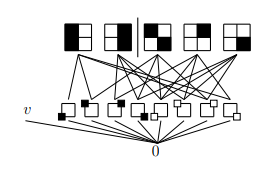
\includegraphics[width=5cm]{M.png} }}%
    \qquad
    \subfloat[graph of M*]{{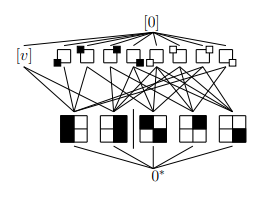
\includegraphics[width=5cm]{Mast.png} }}%
    \caption{The master algebra and the dual algebra}%
    \label{fig:example}%
\end{figure}

\

In figure (1), we can see that $v$ is edged to the two positive examples of our training set. Atoms of $M$ ($0$) are now the duals-of-atoms of M ([$0$]) and $M^{\ast}$'s own atoms ($0^{\ast}$) are also represented.

\subsection{Atomized models}

\subsubsection{Defining the $\boldsymbol{GL}^{\boldsymbol{a}}$ set}

To help formalization, $\boldsymbol{C}(S)$ and $\boldsymbol{A}(S)$ respectively refers to the subset of constants and atoms of a set $S$. Note that $\boldsymbol{C}(M)$ and $\boldsymbol{A}(M)$ can also apply to a model $M$.

\

The lower segement $\boldsymbol{L}$ of an element $x$ is $\boldsymbol{L}(x) = \{y | y \leq x\}$.

\

To distinguish an algebra from its graph we use the prefix $\boldsymbol{G}$, so the lower segement for the graph is defined as $\boldsymbol{GL}(x) = \{ y | (y \rightarrow x) \lor (y = x)\}$

\i

$\boldsymbol{GL}(x)$ therefore contains all the elements edged to $x$ from the "lower" side of the graph.

\

Finaly a superscrit $a$ is used to denote the intersection with the atoms; and we get the final $\boldsymbol{GL}^{\boldsymbol{a}}$ set we will use. 

\

\begin{tcolorbox}
Formaly, for $x \in M$:
\begin{equation}
    \boldsymbol{GL}^{\boldsymbol{a}}(x) = \boldsymbol{GL}(x) \cap \boldsymbol{A}(M)
\end{equation}
\end{tcolorbox}

\

Therefore, $\boldsymbol{GL}^{\boldsymbol{a}}(x)$ is simply the intersection between the elements that are lower than $x$ and all the atoms of a model $M$: \textbf{so we end up geting the atoms that are edged to $x$}.

\

One important thing to point out, is the case of atoms \textbf{in M} ($x \in \boldsymbol{A}(M)$) because we then have $\boldsymbol{GL}(x) = \emptyset$ (by definition of the atoms) and so $\boldsymbol{GL}^{\boldsymbol{a}}$ becomes the set of all atoms of $M$:

\

\begin{tcolorbox}
\begin{equation}
    \forall \phi \in \boldsymbol{A}(M), \boldsymbol{GL}^{\boldsymbol{a}}(\phi) = \boldsymbol{A}(M)
\end{equation}
\end{tcolorbox}

\

\subsubsection{Formal definition of the merge operation in an atomized model}

\

Equation (2) defines how to derive the partial order from the transitive, noncommutative edge relation $\rightarrow$ and atoms. \textbf{A model for which there is a description of the partial order in terms of a set of atoms is an \underline{atomized} model}.

\

Even if we know how to derive the partial order from the atoms and edges, we have not yet a definition for the idempotent operator. 

\

In order to have a more formal definition of the idempotent operator, we can use the set $\boldsymbol{GL}^{\boldsymbol{a}} (x)$ that is defined, as always, only when the graph is transitively closed. 

\

\begin{tcolorbox}
\underline{Definition}: The merge of $a$ and $b$ is the element $a \odot b$ which verifies:

\begin{equation}
    \boldsymbol{GL}^{\boldsymbol{a}}(a \odot b) = \boldsymbol{GL}^{\boldsymbol{a}}(a) \cup \boldsymbol{GL}^{\boldsymbol{a}}(b)
\end{equation}

$\odot$ is therefore the binary operation defined by:

\begin{equation*}
    a \odot b = c \Leftrightarrow \boldsymbol{GL}^{\boldsymbol{a}}(c) = \boldsymbol{GL}^{\boldsymbol{a}}(a) \cup \boldsymbol{GL}^{\boldsymbol{a}}(b)
\end{equation*}

\end{tcolorbox}

Because the idempotent operator becomes a trivial set union of atoms it is clear that this operation is idempotent, commutative and associative. It is also consistent with
the partial order given in equation (2):

\begin{equation*}
    (a \odot b = b) \Leftrightarrow (a < b) \Leftrightarrow (\forall \phi, ((\phi \not\rightarrow a) \lor (\phi \rightarrow b)))
\end{equation*}

\

From these equivalences the relationship between the partial order and $\boldsymbol{GL}^{\boldsymbol{a}}$ is clear that $a < b \Leftrightarrow \boldsymbol{GL}^{\boldsymbol{a}}(a) \cup \boldsymbol{GL}^{\boldsymbol{a}}(b) = \boldsymbol{GL}^{\boldsymbol{a}}(b) \Leftrightarrow \boldsymbol{GL}^{\boldsymbol{a}}(a) \subset \boldsymbol{GL}^{\boldsymbol{a}}(b)$; so:

\

\begin{mybox}{red}{\textbf{Proprety 1 of $\boldsymbol{GL}^{\boldsymbol{a}}$}}


\begin{equation}
    a < b \Leftrightarrow \boldsymbol{GL}^{\boldsymbol{a}}(a) \subset \boldsymbol{GL}^{\boldsymbol{a}}(b)
\end{equation}

\end{mybox}

\

[\colorbox{green}{\textbf{Note}} The use of a strict $\subset$ is not consistant with the idempotent proprety $x \odot x = x$ because $x \odot x = x \Leftrightarrow x < x \Leftrightarrow \boldsymbol{GL}^{\boldsymbol{a}}(x) \subset \boldsymbol{GL}^{\boldsymbol{a}}(x)$ is technically false when it should be true, given that $x < x \Leftrightarrow \forall \phi, (\neg(\phi \rightarrow x) \lor (\phi \rightarrow x)) = \top$. This might just be a choice of notations but in that case $\subset$ should be understood as $\subseteq$ ]

\

For our images problem, we want a model for which $v$ is a set included in the positive training images, $T_1^+$ and $T_2^+$ as 

\begin{equation*}
    v < T_i^+ \Leftrightarrow \boldsymbol{GL}^{\boldsymbol{a}}(v) \subset \boldsymbol{GL}^{\boldsymbol{a}}(T_i^+)
\end{equation*}

We will also be looking for a particular atomic model for which the atoms of constant $v$ are not all in the terms corresponding with negative training examples:

\begin{equation*}
    v \not< T_i^- \Leftrightarrow \boldsymbol{GL}^{\boldsymbol{a}}(v) \not\subset \boldsymbol{GL}^{\boldsymbol{a}}(T_i^-)
\end{equation*}

\subsection{Trace and trace constrains}

\subsubsection{Definitions and propreties}

The trace is central for the embedding procedure as a guiding tool for algebraic transformations.
By operating the algebra while keeping the trace of some elements invariant, we can control the global effects caused by our local changes.

\

The trace \textbf{Tr}$(x)$ maps an element $x \in M$ to a set of atoms in $M^{\ast}$. To calculate the trace of $x$, we find its atoms in the graph of $M$ ($\boldsymbol{GL}^{\boldsymbol{a}}(x)$); since atoms are minima of $M$, dual-of-atoms are maxima of $M^{\ast}$, so for each atom $\phi_i$ of $x$ there is a dual-of-atom at the top of the graph of $M^{\ast}$, [$\phi_i$]. Each of these [$\phi_i$] also have an associated set of atoms in $M^{\ast}$, $\boldsymbol{GL}^{\boldsymbol{a}}([\phi_i])$. The trace of $x$ is defined as the intersection all the atoms of $[\phi_i]$ in $M^{\ast}$. Formaly:

\

\begin{tcolorbox}

For $x \in M$, the trace of $x$ is defined as:

\begin{equation}
    \textbf{Tr}(x) = \bigcap_{\phi \in \boldsymbol{GL}^{\boldsymbol{a}}(x)} \boldsymbol{GL}^{\boldsymbol{a}}([\phi])
\end{equation}
\end{tcolorbox}

\

Here are some propreties of the trace:

\

\begin{mybox}{red}{\textbf{Proprety 1 of the trace}}

\begin{equation}
    \textbf{Tr}(a \odot b) = \textbf{Tr}(a) \cap \textbf{Tr}(b)
\end{equation}

\end{mybox}

\noindent
\underline{Proof:}

\begin{align*}
    \textbf{Tr}(a \odot b) &= \bigcap_{\phi \in \boldsymbol{GL}^{\boldsymbol{a}}(a \odot b)} \boldsymbol{GL}^{\boldsymbol{a}}([\phi]) \\
    &= \bigcap_{\phi \in \boldsymbol{GL}^{\boldsymbol{a}}(a) \cup \boldsymbol{GL}^{\boldsymbol{a}}(b)} \boldsymbol{GL}^{\boldsymbol{a}}([\phi]) \\
    &= \bigcap_{\phi \in \boldsymbol{GL}^{\boldsymbol{a}}(a)}  \boldsymbol{GL}^{\boldsymbol{a}}([\phi])\text{    } \cap \bigcap_{\psi \in \boldsymbol{GL}^{\boldsymbol{a}}(b)} \boldsymbol{GL}^{\boldsymbol{a}}([\psi]) \\
    &= \textbf{Tr}(a) \cap \textbf{Tr}(b)
\end{align*}

\

\begin{mybox}{red}{\textbf{Proprety 2 of the trace}}

\begin{equation}
    a < b \Rightarrow \textbf{Tr}(b) \subset \textbf{Tr}(a)
\end{equation}

\end{mybox}

\noindent
\underline{Proof:}

\

From (2) we have:

\begin{equation*}
    a < b \Leftrightarrow a \odot b = b
\end{equation*}

And from the proprety (1) of the trace:

\begin{equation*}
    a \odot b = b \Rightarrow \textbf{Tr}(a \odot b) = \textbf{Tr}(a) \cap \textbf{Tr}(b) = \textbf{Tr}(b)
    \Rightarrow \textbf{Tr}(b) \subset \textbf{Tr}(a)
\end{equation*}

\

This makes a correspondence between order relations in $M$ and trace interrelations between $M$ and $M^{\ast}$ that are called \textbf{trace constrains}. For our image problem, we are intrested in obeying trace constrains for the positive training examples, $v < T_i^+$, for which we then need to enforce $\textbf{Tr}(T_i^+) \subset \textbf{Tr}(v)$.

\

For negative training examples, $T_i^-$, we want $\neg(v < T_i^-)$ so we want to enforce $\textbf{Tr}(T_i^-) \not\subset \textbf{Tr}(v)$.

\

\textbf{There is actualy no inplicationryuiop between $\textbf{Tr}(T_i^+) \subset \textbf{Tr}(v)$ and $v < T_i^+$} (given that there is no equivalence) \textbf{but} this still provides a necessary starting point, giving that once the trace constraint is met, no transformation of $M$ can produce $v < T_i^-$:

\begin{equation}
    \textbf{Tr}(T_i^-) \not\subset \textbf{Tr}(v) \Rightarrow \neg(v < T_i^-)
\end{equation}

[\colorbox{green}{\textbf{Note}}: Authors say that this inclusion does not follow from (9), yet it seems to be the contraposition of (11), which follows from (1) and (10), wich does follow from (9):]

\

\

\underline{Page 11-12:}
\textit{
While the operator [ ] does not really map M into its dual semilattice, the traces of the
elements of M form an algebra that very much resembles the dual of M. This new algebra has
trace constraints in the place of order relations and set intersections in the place of set unions.
There are still some subtle differences between a proper dual of M and the dual algebra provided
by the trace. For example, the trace is defined with the atoms of M instead of the constants
of M, so it depends on the particular atomization of M. While finding a proper dual of M
amounts in difficulty to calculate M itself, enforcing the trace constraints is easier because we
have the extra freedom of introducing new atoms in M. In addition, we do not have restrictions
for the size of the traces. We do not care if the traces are large or small.
We want an atomization for $M$ but first we have to calculate an atomization for $M^{\ast}$. The
atomization we are going to build for $M$ does not correspond with the dual of $M^{\ast}$
, neither it
corresponds with the dual of the algebra defined by the trace. It corresponds with an algebra
freer than the algebra described by the traces. In Section 3.4 we explain the role that algebraic
freedom plays as a counterbalance to cardinal minimization.
}

\

\subsubsection{Enforcing trace constrains}

\

\noindent
\textbf{\underline{A first optional step}}

\

To enforce trace constrains we can start, although this step is optinal, by enforcing \\ $\neg([T_i^-] < [v])$ by adding an atom to $[T_i^-]$ in $M^{\ast}$ so we enforce $\neg(v < T_i^-)$ in M.

\

In our image exemple, for every negative example $T_i^-$ we add atoms $\zeta_i$, $i \in [|1,3|]$, so that $\forall i \in [|1,3|], \zeta_i \rightarrow [T_i^-]$:

\begin{center}
    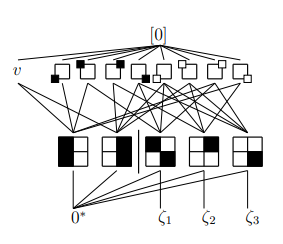
\includegraphics[scale = 0.7]{enforcing.png}
\end{center}

The new atoms are not in $\boldsymbol{GL}^{\boldsymbol{a}}([v])$ so the reverted negative relations are satisfied:

\begin{equation*}
    \neg([T_i^-] < [v]) \Leftrightarrow \boldsymbol{GL}^{\boldsymbol{a}}([T_i^-]) \not\subset \boldsymbol{GL}^{\boldsymbol{a}}([v]) = \{0^{\ast},\zeta_i \} \not\subset \{ 0^{\ast} \}
\end{equation*}

\

In fact all reverted relations, positive and negative, are satisfied at this point (remenber that for the authors $\subset$ means $\subseteq$).

\begin{equation*}
    [v] < [T_i^+] \Leftrightarrow \boldsymbol{GL}^{\boldsymbol{a}}([v]) \subset \boldsymbol{GL}^{\boldsymbol{a}}([T_i^+]) = \{0^{\ast}\} \subset \{ 0^{\ast} \}
\end{equation*}

\

\noindent
\textbf{\underline{Preprocessing}}

\

We have now the chance to detect if the input order relations are inconsistent. First, we make sure that for each couple of terms $T_1$ and $T_2$ mentionned in the input order relations such that the component constants of $T_1$ are a subset of those of $T_2$ we have added the edge $[T_2] \rightarrow [T_1]$.

\

If there are edges pointing in both directions \colorbox{green}{?} between two elements of $M^{\ast}$ we can identify them as the same element. \textbf{Two or more elements of $M$ may share the same dual}. 

\

This completes the preprocessing step that speeds up the enforcing of the trace constrains and validates the consistency of the embedding.

\

\noindent
\textbf{\underline{Enforcing the trace constrains}}

\

We can now enforce trace constrains for the negative examples, $\textbf{Tr}(T_i^-) \not\subset \textbf{Tr}(v)$. To compute the trace, we place the graph for $M$ and for $M^{\ast}$ side to side, to left and right respectively.

\begin{center}
    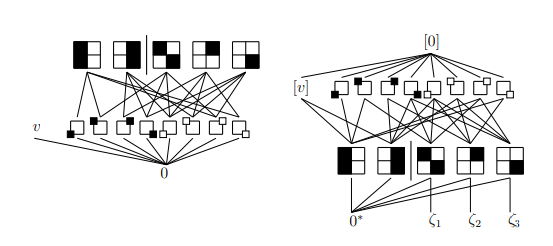
\includegraphics[scale = 0.7]{algorithm.png}
\end{center}

We start with the negative trace constrains. The trace for the negative training examples is
$\textbf{Tr}(T_i^-) = \boldsymbol{GL}^{\boldsymbol{a}}([0]) = \{0^{\ast}, \zeta_1, \zeta_2, \zeta_3\}$. For constant $v$ we also have $\textbf{Tr}(v) = \boldsymbol{GL}^{\boldsymbol{a}}([0])$, so it does not obeyed $\textbf{Tr}(T_i^-) \not\subset \textbf{Tr}(v)$; \textbf{we need to enforce it}.

\

For this, we need to choose a constant $c \in M$ equal to $v$ or such that $[c]$ recieves edges from $[v]$ and not from $[T_i^-]$. We then need to \textbf{add an atom $\phi \rightarrow c$}. 

\

Note that this constant $c$ has propreties directly fulfuled by $v$ (the case where $c \in M$ is equal to $v$) so we can add $\phi \rightarrow v$ and the corresponding dual-of-atom $[v] \rightarrow [\phi]$ in $M^{\ast}$.

\begin{center}
    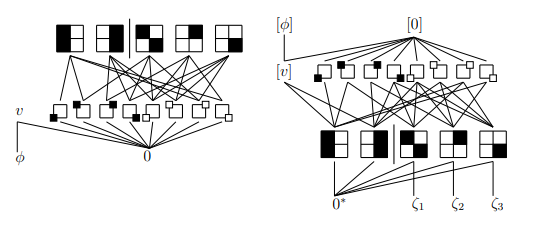
\includegraphics[scale = 0.7]{newatom.png}
\end{center}

Now we have $\textbf{Tr}(T_i^-) = \boldsymbol{GL}^{\boldsymbol{a}}([0]) = \{0^{\ast}, \zeta_1, \zeta_2, \zeta_3\}$ but $\textbf{Tr}(v) = \boldsymbol{GL}^{\boldsymbol{a}}([0]) \cap \boldsymbol{GL}^{\boldsymbol{a}}([\phi]) = \{ 0^{\ast} \}$, because $\boldsymbol{GL}^{\boldsymbol{a}}([\phi]) = \{ 0^{\ast} \}$ so $\textbf{Tr}(T_i^-) = \{0^{\ast}, \zeta_1, \zeta_2, \zeta_3\} \not\subset \textbf{Tr}(v) = \{ 0^{\ast} \}$ is verified.

\

Now, for positive trace constrains, we want $v < T_i^+$ so we need to enforce $\textbf{Tr}(T_i^+) \subset \textbf{Tr}(v)$. First we check if this condition is satisfied: $\textbf{Tr}(T_i^+) = \boldsymbol{GL}^{\boldsymbol{a}}([0]) = \{0^{\ast}, \zeta_1, \zeta_2, \zeta_3\}$ and $\textbf{Tr}(v) = \boldsymbol{GL}^{\boldsymbol{a}}([0]) \cap \boldsymbol{GL}^{\boldsymbol{a}}([\phi]) = \{ 0^{\ast} \}$. The condition is not satisfied.

\

Therefore, we add atoms $\epsilon_i$ to the constants $c_i$ until $\textbf{Tr}(T_i^+)$ equals $\textbf{Tr}(v)$. For the first term $T_1^+$ we just need to edge an atom to the first constant, $\epsilon_1 \rightarrow c_1$; for the secound training example, $T_2^+$ we need to add one atom for each of its constants, $\epsilon_2 \rightarrow c_3$ and $\epsilon_3 \rightarrow c_4$. After imposing the trace constraints the graphs $M$ and $M^{\ast}$ look like this:

\begin{center}
    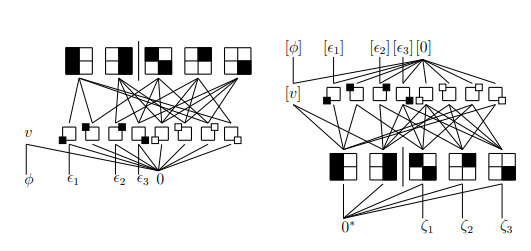
\includegraphics[scale = 0.7]{afterconstrains.png}
\end{center}

Now we have:

\begin{center}
    $\textbf{Tr}(v) = \{0^{\ast}, \zeta_1, \zeta_2, \zeta_3\} \cap \{ 0^{\ast} \} = \{ 0^{\ast} \} $ \\
    $\textbf{Tr}(T_1^+) = \boldsymbol{GL}^{\boldsymbol{a}}([0]) \cap \boldsymbol{GL}^{\boldsymbol{a}}([\epsilon_1]) = \{0^{\ast}, \zeta_1, \zeta_2, \zeta_3\} \cap \{ 0^{\ast} \} = \{ 0^{\ast} \}$ \\
    $\textbf{Tr}(T_2^+) = \boldsymbol{GL}^{\boldsymbol{a}}([0]) \cap \boldsymbol{GL}^{\boldsymbol{a}}([\epsilon_2]) \cap \boldsymbol{GL}^{\boldsymbol{a}}([\epsilon_3]) = \{0^{\ast}, \zeta_1, \zeta_2, \zeta_3\} \cap \{ 0^{\ast}, \zeta_2 \} \cap \{ 0^{\ast}, \zeta_3 \} = \{ 0^{\ast} \}$
\end{center}

Giving us the desired result: $\textbf{Tr}(T_i^+) \subset \textbf{Tr}(v)$.

\

In practice , enforcing trace constrains is achieved through algorithms (two algorithms; one for positive trace constrains and negative trace constrains) that we will present later.

\subsection{Full and Sparse Crossing operations}

After enforcing the trace constraints, all negative relations $v \not< T_i^-$ are already satisfied in $M$. This will always be the case \colorbox{green}{as long as the trace is unchanged (equation (12))}. To build an atomized model that also satisfies the positive relations $v < T_i^+$, we use the Sparse Crossing operation.

\

This trace-invariant operation replaces
the atoms of $v$ for others that are also in $T_i^+$ without interfering with previously enforced positive or negative relations and without changing the traces of any element of $M$.

\subsubsection{Definition of the crossing operation}

Let's consider two elements $a$ and $b$ with atoms:

\begin{center}
    $\boldsymbol{GL}^{\boldsymbol{a}}(a) = \{ \alpha, \beta, \chi \}$ \\
    $\boldsymbol{GL}^{\boldsymbol{a}}(b) = \{\chi, \delta, \epsilon \}$
\end{center}

and suppose we want to enforce $a < b$. \textbf{Extend the graph appending new atoms and edges as}

\begin{center}
    $\phi, \varphi, \gamma \rightarrow \alpha$ \\
    $\pi, \omega, \theta \rightarrow \beta$ \\
    $\chi', \phi, \pi \rightarrow \chi$ \\
    $\delta', \varphi, \omega \rightarrow \delta$ \\
    $\epsilon', \gamma, \theta \rightarrow \epsilon$
\end{center}

Now close the graph by transitive closure and delete $\alpha, \beta, \chi, \delta$ and $\epsilon$ from the graph. Then it holds that:

\begin{equation*}
    \boldsymbol{GL}^{\boldsymbol{a}}(a) = \{ \phi, \varphi, \gamma, \pi, \omega, \theta \} \subset \boldsymbol{GL}^{\boldsymbol{a}}(b) = \{ \chi', \delta', \epsilon', \phi, \varphi, \gamma, \pi, \omega, \theta \}
\end{equation*}

and therefore $a < b$. This is the \textbf{Full Crossing of $a$ into $b$} and it can represented with the table:

\begin{center}
\begin{tabular}{ c|c|c|c } 
 & $\chi$ & $\delta$ & $\epsilon$ \\ 
 \hline
 & $\chi'$ & $\delta'$ & $\epsilon'$ \\
 \hline
 $\alpha$ & $\phi$ & $\varphi$ & $\gamma$\\ 
 \hline
 $\beta$ & $\pi$ & $\omega$ & $\theta$\\ 
\end{tabular}
\end{center}

We say that we have ”crossed” atoms $\alpha$ and $\beta$ into $b$. Note that the first square in the first line of the table is blank because there is no need to "cross" atom $\chi$ of $a$ as it is already in $b$.

\

Crossing made so that $b$ now shares all atoms that are edged to $a$, plus the initial atoms (though they are not quite the same) in $\boldsymbol{GL}^{\boldsymbol{a}}(b)$.

\

In practice, since the crossing is an expensive operation that multiplies the number of atoms, we instead do a Sparse Crossing. The idea is that, as long as we check that all involved atoms remain trace-invariant, the Sparse Crossing operation still enforces $a < b$ and preserves all positive relations. In addition, it also preserves negative relations as long as they are ”protected” by its corresponding negative trace constraint. Details of how sparse crossing works will be given later.

\subsubsection{Full crossing operation propreties}

Formaly, the full crossing operation transforms one graph into another and after transitive closure, it also maps one algebra into another. This mapping function commutes with both operators $\odot$ and [ ] so it is a homomorphism, which gives us one proprety of the full crossing operation:

\

\begin{mybox}{red}{\textbf{Proprety 1 of full crossing}}
The full crossing operator is a homomorphism of the graph algebra, ie. if we call $f$ the mapping function of full crossing:

\begin{equation}
    \forall a,b \in M/\boldsymbol{A}(M), f(a \odot b) = f(a) \odot f(b) 
\end{equation}

We cannot take atoms into consideration, given that full crossing removes some atoms out of the graph.


\

\textbf{This formula means that if $a \odot b = c$ is true in $M$ then it will also be true after full crossing.}

\

Given that $<$ is defined from $\odot$, we immediately get a corollary of this proposition:

\begin{equation}
    \forall a,b \in M/\boldsymbol{A}(M), f(a < b) = f(a) < f(b) 
\end{equation}


\end{mybox}

\noindent
\underline{Proof}:

\

Let $T, c_1$ and $c_2$ be elements of $M/\boldsymbol{A}(M)$ such that $T = c_1 \odot c_2$. We want to prove that the full crossing operation of element $a$ into $b$ does not change the fact that $T = c_1 \odot c_2$. Because of the definition of $\odot$ (equation (7)), we know that:

\begin{equation*}
    T = c_1 \odot c_2 \Leftrightarrow \boldsymbol{GL}^{\boldsymbol{a}}(T) = \boldsymbol{GL}^{\boldsymbol{a}}(c_1) \cup \boldsymbol{GL}^{\boldsymbol{a}}(c_2)
\end{equation*}

\begin{center}
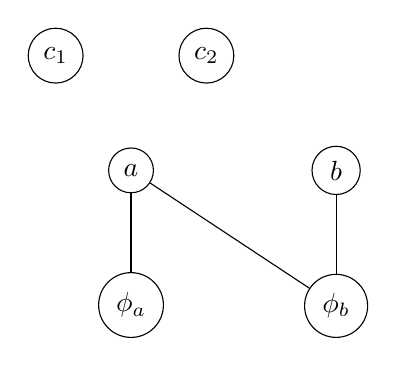
\begin{tikzpicture}[main/.style = {draw, circle}] 
\node[main] (1) {$a$};
\node[main] (2) [right=2cm of 1] {$b$};
\node[main] (3) [below=1cm of 1] {$\phi_a$};
\node[main] (4) [below=1cm of 2] {$\phi_b$};
\node[main] (5) [above left=1cm and 0.5cm of 1] {$c_1$};
\node[main] (6) [above right=1cm and 0.5cm of 1] {$c_2$};

\draw (3) -- (1);
\draw (4) -- (2);
\draw (4) -- (1);
\end{tikzpicture}
\end{center}

\

\begin{mybox}{red}{\textbf{Proprety 2 of full crossing -- \underline{Theorem 1}}}
Full crossing of $a$ into $b$ leaves the trace of all atoms unchanged if and only if the positive trace constraint for $a < b$, ie. $\textbf{Tr}(b) \subset \textbf{Tr}(a)$ is satisfied. 

\

Formaly, if $f$ is the mapping function of full crossing of $a$ into $b$:

\begin{equation}
    \forall \phi \in \boldsymbol{A}(M), \textbf{Tr}(f(\phi)) = \textbf{Tr}(\phi) \Leftrightarrow \textbf{Tr}(b) \subset \textbf{Tr}(a)
\end{equation}

\end{mybox}

\noindent
\underline{Proof}:

\

Let $a$ and $b$ be to elements of the graph.
Let $\Phi$ be the set of atoms involved in the full crossing of $a$ \textbf{in} $b$. $\Phi$ is entirely defined as:

\begin{equation*}
    \Phi = \boldsymbol{GL}^{\boldsymbol{a}}(a) \Delta \boldsymbol{GL}^{\boldsymbol{a}}(b)
\end{equation*}

Where $\Delta$ is the symmetric difference of sets.

\

For each $\phi \in \Phi$; crossing of $a$ in $b$ will result in the creation of a family of atoms $(\phi_j)_{j\in N}$ such that $\phi = \bigodot_j \phi_j$. 

\

Before crossing $\phi$ is a minima and by definition $\textbf{Tr}(\phi) = \boldsymbol{GL}^{\boldsymbol{a}}([\phi])$. After the crossing the new minima are $(\phi_j)$ and so $\textbf{Tr}(\bigodot_j \phi_j) = \bigcap_j \boldsymbol{GL}^{\boldsymbol{a}}([\phi_j])$. The left side of the equivalence therefore becomes:

\begin{equation*}
    \forall \phi \in \Phi, \boldsymbol{GL}^{\boldsymbol{a}}([\phi]) = \bigcap_j \boldsymbol{GL}^{\boldsymbol{a}}([\phi_j])
\end{equation*}

Since $\phi$ is not in both $a$ and $b$, we have either $(\phi < a)\land \neg(\phi < b)$ or $\neg(\phi < a)\land (\phi < b)$; meaning we have either $\phi$ edged to $a$ or $\phi$ edged to $b$.

\

\noindent
\underline{if $\phi$ is edged to $b$:}

\

\textbf{An atom $\phi$ initialy edged to $b$ always has a corresponding element $\phi'$ edged only to $\phi$}; meaning that the family that is edged to $\phi$ contains one atom $\phi'$ that verifies: $\boldsymbol{GL}^{\boldsymbol{a}}([\phi']) = \boldsymbol{GL}^{\boldsymbol{a}}([\phi])$. In addition, because atoms $\phi_j$ can only be edged to $a$ and $b$ (or stricly $b$); we always have more (or stricly the same) atoms in $\boldsymbol{GL}^{\boldsymbol{a}}([\phi_j])$ than we have in $\boldsymbol{GL}^{\boldsymbol{a}}([\phi'])$. So:

\begin{equation*}
    \forall \phi_j, \boldsymbol{GL}^{\boldsymbol{a}}([\phi']) \subset \boldsymbol{GL}^{\boldsymbol{a}}([\phi_j]) \Rightarrow \bigcap_j \boldsymbol{GL}^{\boldsymbol{a}}([\phi_j]) = \boldsymbol{GL}^{\boldsymbol{a}}([\phi']) = \boldsymbol{GL}^{\boldsymbol{a}}([\phi])
\end{equation*}

\

From the previous equation we get the desired result \textbf{with or without $\textbf{Tr}(b) \subset \textbf{Tr}(a)$}:

\begin{equation*}
    \forall \phi \in \boldsymbol{GL}^{\boldsymbol{a}}(b), \boldsymbol{GL}^{\boldsymbol{a}}([\phi]) = \bigcap_j \boldsymbol{GL}^{\boldsymbol{a}}([\phi_j]) \text{ is true for any crossing}
\end{equation*}

\noindent
\underline{if $\phi$ is edged to $a$:}

\

Let's say $b$ was atomized as $b = \bigodot_j \epsilon_j$, before crossing. For each $\epsilon_j$, a new atom $\varphi_j$ is created and edges $(\varphi_j \rightarrow \phi \land \varphi_j \rightarrow \epsilon_j)$ are appended to the graph. New edges are appended to the graph of $M^{\ast}$: $([\phi] \rightarrow [\varphi_j] \land [\epsilon_j \rightarrow [\varphi_j])$. Since no other elements are edged to $[\varphi_j]$, then:

\begin{equation*}
    \boldsymbol{GL}^{\boldsymbol{a}}([\varphi_j]) = \boldsymbol{GL}^{\boldsymbol{a}}([\phi])\cup\boldsymbol{GL}^{\boldsymbol{a}}([\epsilon_j])
\end{equation*}

\

For $j = 1$, we can visualize the situation for a better understanding:

\begin{center}
\begin{tikzpicture}[main/.style = {draw, circle}] 
\node[main] (1) {$a$};
\node[main] (2) [right=2cm of 1] {$b$};
\node[main] (3) [below=1cm of 1] {$\phi$};
\node[main] (4) [below=1cm of 2] {$\epsilon_1$};
\node[main] (5) [right=5cm of 1] {$[\phi]$};
\node[main] (6) [right=2cm of 5] {$[\epsilon_1]$};
\node[main] (7) [below=1cm of 5] {$[a]$};
\node[main] (8) [below=1cm of 6] {$[b]$};
\node[main] (9) [below=1cm of 3] {$\varphi_1$};
\node[main] (10) [above=1cm of 6] {$[\varphi_1]$};

\draw (3) -- (1);
\draw (4) -- (2);
\draw (9) -- (4); 
\draw (9) -- (3); 

\draw (7) -- (5);
\draw (8) -- (6);
\draw (5) -- (10); 
\draw (6) -- (10); 
\end{tikzpicture}
\end{center}

The previous equation then gives us:

\begin{align*}
    \textbf{Tr}(\bigodot_j \varphi_j) &= \bigcap_j \boldsymbol{GL}^{\boldsymbol{a}}([\varphi_j]) \\
    &= \bigcap_j \{ \boldsymbol{GL}^{\boldsymbol{a}}([\phi]) \cup \boldsymbol{GL}^{\boldsymbol{a}}([\epsilon_j])\} \\
    &= \boldsymbol{GL}^{\boldsymbol{a}}([\phi]) \cup \{ \bigcap_j \boldsymbol{GL}^{\boldsymbol{a}}([\epsilon_j])\} \\
    &= \boldsymbol{GL}^{\boldsymbol{a}}([\phi]) \cup \textbf{Tr}(b) 
\end{align*}

This means that (given that before crossing, $\phi$ is a minima and by definition $\textbf{Tr}(\phi) = \boldsymbol{GL}^{\boldsymbol{a}}([\phi])$), $\forall \phi \in  \boldsymbol{GL}^{\boldsymbol{a}}(a)$:

\begin{equation*}
    \textbf{Tr}(f(\phi)) = \textbf{Tr}(\phi) \cup \textbf{Tr}(b)
\end{equation*}

\textbf{In other words: when $\phi$ is crossed into $b$, the trace of $\phi$ gains the set $\textbf{Tr}(b)$. Meaning that $\textbf{Tr}(\phi)$ remains invariant if and only if it contained $\textbf{Tr}(b)$ before crossing.} For a formal proof of the equivalence:

\

\noindent
\underline{Proof of que equivalence}:

\

Let's suppose that $\forall \phi \in \boldsymbol{GL}^{\boldsymbol{a}}(a), \textbf{Tr}(f(\phi)) = \textbf{Tr}(\phi)$; then the previous equation becomes:

\begin{equation*}
    \forall \phi \in \boldsymbol{GL}^{\boldsymbol{a}}(a), \textbf{Tr}(\phi) = \textbf{Tr}(\phi) \cup \textbf{Tr}(b) \Rightarrow \textbf{Tr}(b) \subset \textbf{Tr}(\phi) 
\end{equation*}

By definition:

\begin{equation*}
    \textbf{Tr}(a) = \bigcap_{\phi \in \boldsymbol{GL}^{\boldsymbol{a}}(a)} \textbf{Tr}(\phi)
\end{equation*}

And so we get the final result we were looking for:

\begin{equation*}
    \forall \phi \in \boldsymbol{GL}^{\boldsymbol{a}}(a), \textbf{Tr}(f(\phi)) = \textbf{Tr}(\phi) \Rightarrow \textbf{Tr}(b) \subset \textbf{Tr}(a)
\end{equation*}

\

Let's now suppose that $\textbf{Tr}(b) \subset \textbf{Tr}(a)$; then: 

\begin{equation*}
  \textbf{Tr}(b) \subset \bigcap_{\phi \in \boldsymbol{GL}^{\boldsymbol{a}}(a)} \textbf{Tr}(\phi) \Rightarrow \forall \phi \in \boldsymbol{GL}^{\boldsymbol{a}}(a), \textbf{Tr}(b) \subset \textbf{Tr}(\phi).  
\end{equation*}

So:

\begin{equation*}
    \forall \phi \in  \boldsymbol{GL}^{\boldsymbol{a}}(a), \textbf{Tr}(f(\phi)) = \textbf{Tr}(\phi) \cup \textbf{Tr}(b) = \textbf{Tr}(\phi)
\end{equation*}

\subsubsection{After Sparse Crossing}

After the sparse crossing algorithm is applied in our image example, we get the following state of the algebras:


\begin{center}
    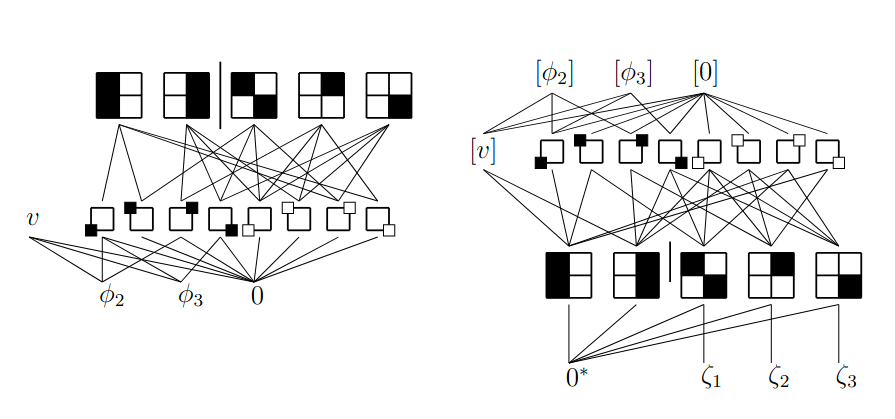
\includegraphics[scale = 0.6]{final_state.png}
\end{center}

The Sparse Crossing operation has worked; the positive training examples all obey $v < T_i^+$ and the negatives ones $v < T_j^-$. The atoms of $v$ are $\boldsymbol{GL}^{\boldsymbol{a}}(v) = \{ 0, \phi_2, \phi_3 \}$ and the atoms for the positive training examples are also $\boldsymbol{GL}^{\boldsymbol{a}}(T_{1,2}^+) = \{ 0, \phi_2, \phi_3 \}$, while for the negative examples we have $\boldsymbol{GL}^{\boldsymbol{a}}(T_{1,3}^-) = \{ 0, \phi_3 \}$ and $\boldsymbol{GL}^{\boldsymbol{a}}(T_2^-) = \{ 0, \phi_2 \}$.


\subsection{Reduction operation}

\colorbox{green}{TODO}

The trace-preserving reduction scheme presented in this section works well in combinationwith Sparse Crossing and finds small, generalizing models efficiently. 

\subsection{Batch training}

So we have seen how to learn an atomized model from a set $R$ of positive and negative examples. In practice, we would check the accuracy of the learned model in test data. If the accuracy is below some desired level, we would continue training with a new set of ewamples. Therefore, rather than having a single set $R$, we have a series of \textbf{batches} $R_0, R_1, ..., R_n$ where the subscript corresponds with the training epoch.



\end{document}



















